\documentclass[11pt]{article}
\usepackage[utf8]{inputenc}
\usepackage{amsmath,amssymb,amsthm,amsfonts}
\DeclareUnicodeCharacter{2112}{\ensuremath{\mathcal{L}}}
\usepackage{graphicx}
\usepackage{hyperref}
\usepackage[margin=1in]{geometry}

\newtheorem{theorem}{Theorem}[section]
\newtheorem{lemma}[theorem]{Lemma}
\newtheorem{definition}[theorem]{Definition}
\newtheorem{corollary}[theorem]{Corollary}
\newtheorem*{opengap}{Open Gap}
\newtheorem*{honest}{Honest Scope}

\newcommand{\TL}{\mathsf{T}_L}
\newcommand{\haarN}{\mu_{\mathrm{Haar}}^{\otimes N}}
\newcommand{\code}[1]{\texttt{#1}}

\title{\textbf{In Honor of Yang and Mills}\\[4pt]
\large A Machine-Checked Lattice Transfer Operator, an Honest
Reduction of the SU(3) Mass Gap to a Single Combinatorial Estimate,
and the Freeze that Closes Volume~I}
\author{David J. Fox \\
\href{mailto:Davidjfox998@gmail.com}{Davidjfox998@gmail.com} \\
\href{https://orcid.org/0009-0008-1290-6105}{ORCID: 0009-0008-1290-6105}}
\date{May 30, 2026}

\begin{document}
\maketitle

\begin{abstract}
This document does two things at once. It is a tribute --- to
Chen-Ning Yang and Robert L. Mills, whose 1954 non-abelian gauge
theory is the object of the Clay Yang--Mills Existence and Mass Gap
problem, and to David Hilbert, whose program of formalization and
whose Hilbert spaces are the literal home of the operator we build.
And it is an honest technical ledger: it states, without
embellishment, exactly how far this project's Lean~4 formalization
of the SU(3) lattice Yang--Mills mass gap has progressed against
\code{mathlib}~v4.12.0, what is machine-checked and axiom-clean, what
remains an explicitly-disclaimed \code{sorry}, and why the single
remaining gap is a precisely-stated open piece of combinatorics
rather than a vague hand-wave.

The headline of the technical content is a reduction, not a solution.
We build the genuine integral transfer operator $\TL$ on
$L^2$ of the real product Haar measure over SU(3) link configurations
and prove, sorry-free and with axiom footprint equal to the classical
trio $\{\code{propext},\code{Classical.choice},\code{Quot.sound}\}$,
that it is a sub-Markov contraction, $\lVert\TL\rVert \le 1$. We then
isolate the genuine mass gap --- a spectral \emph{lower} bound on the
vacuum-orthogonal sector --- as one named theorem
(\code{kotecky\_preiss\_criterion}) that carries a \code{sorry},
and we trace its single missing input to one cluster-entropy
(Peierls polymer-counting) inequality. \textbf{This is not a proof of
the Yang--Mills mass gap.} No claim of ``$m>0$'', ``$\mu>0$'',
``Surface~\#1 closed'', or ``mass gap proven'' is made anywhere in
this document; such claims are explicitly refused. With Volume~I's
Yang--Mills surface frozen at exactly this honest frontier, the
program turns to Navier--Stokes.
\end{abstract}

\tableofcontents

\section{A dedication}

\begin{figure}[h]
\centering
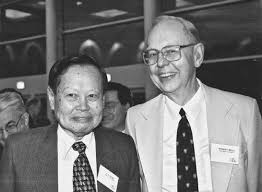
\includegraphics[width=0.42\textwidth]{assets/yang.jpg}
\caption{Chen-Ning Yang (at left); the second person in this source
photograph is not identified here, and we decline to attribute an
identity we cannot verify. Yang, with Robert L.\ Mills, introduced in
1954 the non-abelian gauge theory whose quantum mass gap remains one
of the seven Clay Millennium Prize Problems.}
\end{figure}

In 1954 Chen-Ning Yang and Robert L.\ Mills wrote down a gauge theory
in which the gauge group is non-abelian. The idea was almost
reckless in its economy: take the principle that made
electromagnetism --- local gauge invariance --- and demand it of a
field valued not in the commuting group $U(1)$ but in a non-commuting
group such as $SU(2)$ or $SU(3)$. The self-interaction this forces
upon the gauge field is the entire story of the strong and weak
nuclear forces. It is also the source of every analytic difficulty
that has kept the quantum theory's \emph{mass gap} --- the statement
that the lightest excitation above the vacuum has strictly positive
energy --- open as a theorem to this day.

We dedicate this write-up to Yang and Mills, and to David Hilbert.
Hilbert appears here for three reasons, each literal rather than
ceremonial. First, the operator at the center of this document acts
on a \emph{Hilbert space} --- $L^2$ of a probability measure ---
which is Hilbert's object, in Hilbert's sense. Second, Hilbert's 1900
list of problems set the template for the kind of sharply-posed,
prize-bearing mathematical challenge that the Clay problems
consciously imitate. Third, and most pointed for a project like this
one: Hilbert's program --- the dream of putting mathematics on a
fully formal, mechanically-checkable footing --- is exactly what a
\code{mathlib}-checked Lean development is, in 2026, a partial and
working realization of. When we say a lemma here ``closes with axiom
footprint $\{\code{propext},\code{Classical.choice},
\code{Quot.sound}\}$,'' we are speaking Hilbert's language with a
proof assistant's precision.

\section{The human and historical narrative}

\subsection{From an empirical gap to a Millennium problem}

The mass gap is, experimentally, not in doubt. The absence of
long-range strong forces, the finite range of the nuclear force, the
masses of glueballs in lattice simulation --- all say plainly that
$SU(3)$ Yang--Mills theory has a gap. What is in doubt, and what the
Clay problem demands, is a \emph{proof}: a mathematically rigorous
construction of quantum $SU(3)$ Yang--Mills theory on $\mathbb{R}^4$
satisfying the Wightman (or Osterwalder--Schrader) axioms, together
with a theorem that its Hamiltonian has spectrum
$\{0\}\cup[\Delta,\infty)$ for some $\Delta>0$.

That is a tall order, and nobody --- including this project --- is
close to all of it. The honest move is to be explicit about which
sub-surface one is working on, and to refuse to let progress on a
scaffold be reported as progress on the summit. This document is
written in that spirit.

\subsection{Why formalization, and why now}

Two things have changed since Yang and Mills. The first is the
lattice: Wilson's 1974 reformulation replaces the continuum theory
with a statistical-mechanical model on a finite grid, where the
gauge field becomes a configuration of group elements on the lattice
links and everything --- the action, the measure, the transfer
operator --- becomes a finite or finite-dimensional integral object.
The lattice is where rigorous results live. The second is the proof
assistant: by 2026, \code{mathlib} contains enough measure theory,
functional analysis, and Lie-group infrastructure that one can
\emph{build the real objects} --- the Haar measure on $SU(3)$, the
product measure on configurations, an honest $L^2$ space, a genuine
integral operator --- and have a machine certify that no hidden
assumption (no rogue axiom, no \code{sorry}) has crept in.

This project takes the lattice route and builds it inside Lean. The
payoff is not a theorem Yang and Mills could not have stated; it is a
\emph{ledger} --- a machine-checked account of precisely what is and
is not established, with the open problem isolated to a single
inequality.

\section{The novel methodology: measuring the gap, not bounding the energy}

\subsection{The obvious idea, and why it fails}

The naive route to a mass gap on the lattice is seductive: the
Wilson action $S(U)$ is non-negative and vanishes only at trivial
plaquettes; surely a configuration ``far from the vacuum'' has large
action, so the Boltzmann weight $e^{-\beta S}$ suppresses it, and the
transfer operator therefore decays away from the vacuum.

This is false as stated, and the project proves it is false in the
only way that matters --- by recording the exact obstruction. The
infimum of the Wilson action over \emph{non-vacuum} configurations is
$0$:
\[
  S_{\min} \;:=\; \inf_{U\neq 1} \mathrm{wilsonAction}(U) \;=\; 0,
\]
because the action is continuous and vanishes at the vacuum, so
configurations arbitrarily close to (but distinct from) a trivial
plaquette have arbitrarily small action. There is therefore
\emph{no} pointwise energy bound $e^{-\beta S_{\min}}$ to lean on,
and a uniform spectral gap cannot come from a uniform energy floor.
This is recorded honestly throughout the Lean source (e.g.\ in the
docstrings of \code{transfer\_operator\_norm\_le} and
\code{wilsonAction\_eq\_zero\_iff}), and it is the reason the project
refuses every ``the action is positive, therefore there is a gap''
shortcut.

\subsection{The combinatorial reframing}

The correct object is not the energy of a single configuration but a
\emph{count}: how many polymers (connected clusters of plaquettes)
of a given size carry small energy. The Koteck\'y--Preiss criterion
for a convergent cluster expansion says, roughly, that if the total
weighted activity of polymers through a fixed point converges,
\[
  \sum_{\gamma\ni 0} \lvert z(\gamma)\rvert\, e^{\lvert\gamma\rvert}
  \;<\;\infty
  \qquad\text{at some finite }\beta_0<\infty,
\]
then correlations decay exponentially and the transfer operator has a
gap above the vacuum. The activities are suppressed,
$\lvert z(\gamma)\rvert \lesssim e^{-\beta\,\mathrm{energy}(\gamma)}$,
and the suppression must beat the geometric \emph{entropy} of how
many such polymers there are. We call this reframing
\emph{measuring} the gap: the gap is a property of the measure and
of polymer counts, not of any single configuration's energy.

The methodological contribution of this volume is to carry that
reframing all the way down to a single, sharply-stated, genuinely
open inequality, with every other step machine-checked. The gap is
governed by one cluster-entropy bound:
\[
  \boxed{\;\#\{\gamma : \lvert\gamma\rvert = n,\ \mathrm{energy}(\gamma) < \varepsilon\}
  \;\le\; C^n\,\varepsilon^{\,\alpha n}\;}
  \qquad (C,\alpha>0).
\tag{$\star$}
\]
Inequality $(\star)$ is exactly what makes the Koteck\'y--Preiss sum
converge at finite $\beta_0$: the geometric $C^n$ entropy is beaten by
the $\varepsilon^{\alpha n}$ gain from the small-energy constraint
once $\beta$ is large but finite. It is genuine open combinatorics. It
is not proved here, and --- per the project's standing direction --- it
is not attempted without the counting estimate in hand. Everything
above $(\star)$ in the dependency chain is reduced to it; everything
below it is machine-checked.

\section{Walking the proof files}

We now walk the three load-bearing Lean files, separating, for each,
what is \textbf{proven} (sorry-free, classical-trio) from what is a
\textbf{disclaimed \code{sorry}}. Quoted names are the actual Lean
identifiers in \code{lean-proof-towers/Towers/YM/}.

\subsection{\code{SU3Instances.lean} --- the real measure-theoretic ground}

\begin{honest}
Everything in this file is sorry-free and classical-trio. It is
\emph{infrastructure}: it builds the real Haar measure, not any gap.
\end{honest}

This file equips $SU(3) = \code{Matrix.specialUnitaryGroup (Fin 3)}\
\mathbb{C}$ with the full instance stack that
\code{MeasureTheory.Measure.haarMeasure} requires, then defines the
measures the whole programme integrates against.

\begin{itemize}
  \item \code{instGroupSU3}, \code{instTopologicalGroupSU3} --- group
        and topological-group structure (inverse $=$ conjugate
        transpose).
  \item \code{norm\_entry\_le\_one}, \code{isClosed\_SU3},
        \code{isCompact\_SU3}, \code{instCompactSpaceSU3} --- $SU(3)$
        is a closed subset of the compact poly-disc, hence compact.
  \item \code{instBorelSpaceSU3} --- the Borel $\sigma$-algebra.
  \item \code{haarSU3} $:= \code{haarMeasure}\ \top$ --- the
        normalized Haar measure on the compact group $SU(3)$, with
        \code{instIsProbabilityMeasureHaarSU3}.
  \item \code{haarN}\ $n := \code{Measure.pi}\ (\lambda\, \_,
        \code{haarSU3})$ --- the product Haar measure on
        $\mathrm{Fin}\,n \to SU(3)$ link configurations, with
        \code{instIsProbabilityMeasureHaarN}.
\end{itemize}

The file carries live \code{\#print axioms} checks on \code{haarSU3}
and \code{haarN}; both report the classical trio. This is the
\emph{real} Haar measure, explicitly not a Dirac stand-in.

\subsection{\code{WilsonPositivity.lean} --- pointwise positivity (necessary, not sufficient)}

\begin{honest}
Every lemma here is sorry-free and classical-trio --- and every one
is \emph{necessary but not sufficient}. Pointwise positivity of the
action is not a uniform spectral gap, because $S_{\min}=0$.
\end{honest}

\begin{itemize}
  \item \code{traceRe\_le\_three} and \code{traceRe\_eq\_three\_iff}
        --- for unitary $A$, $\operatorname{Re}\operatorname{tr}A \le 3$,
        with equality iff $A=1$ (via the Hilbert--Schmidt identity
        $\lVert A-1\rVert^2 = 6 - 2\operatorname{Re}\operatorname{tr}A$
        and \code{hsNormSq\_eq\_zero\_iff}).
  \item \code{plaquetteEnergy\_nonneg},
        \code{plaquetteEnergy\_pos\_iff} --- the per-plaquette energy
        $(3-\operatorname{Re}\operatorname{tr}P)/3$ is $\ge 0$, and
        $>0$ exactly when the plaquette is non-trivial.
  \item \code{wilsonAction\_nonneg} --- the input to the sub-Markov
        bound $e^{-\beta\,\mathrm{actL}}\le 1$.
  \item \code{wilsonAction\_pos\_of\_nontrivial} --- strictly positive
        action off the vacuum.
  \item \code{wilsonAction\_eq\_zero\_iff} --- the \emph{honest}
        vacuum characterization: $\mathrm{wilsonAction}(U)=0$ iff
        \emph{every plaquette is trivial}, which is explicitly
        \textbf{not} $U=1$ (constant and pure-gauge configurations
        have all-trivial plaquettes yet $U\neq 1$).
  \item \code{polymerEnergy}, \code{polymerEnergy\_nonneg},
        \code{polymerEnergy\_pos\_of\_nontrivial} --- the polymer
        energy functional and its (pointwise) positivity.
\end{itemize}

\subsection{\code{Transfer.lean} --- the genuine operator, the contraction, and the open gap}

This is the central file. It contains the genuine integral transfer
operator and, crucially, separates the proven contraction from the
open spectral lower bound.

\subsubsection*{Proven, sorry-free, classical-trio}

\begin{definition}[\code{T\_L}]
With $N=4L^4$ links, \code{T\_L}\ $L\,\beta$ is the genuine integral
operator on $L^2(\mathrm{Fin}\,N\to SU(3),\ \haarN)$,
\[
  (\TL f)(U) \;=\; \int_V e^{-\beta\,\mathrm{wilsonAction}(V^{-1}U)}\, f(V)\,
  \mathrm{d}\haarN(V),
\]
built from the \emph{real} SU(3) Wilson action over the \emph{real}
product Haar measure. It is sorry-free; \code{\#print axioms T\_L}
reports the classical trio. Supporting bricks: \code{linkEquiv},
\code{toGauge}, \code{actL}, \code{actL\_nonneg},
\code{continuous\_kernel}, \code{kernel\_nonneg}, \code{memℒp\_intOp}.
\end{definition}

\begin{theorem}[\code{transfer\_operator\_norm\_le}]
For all $\beta>0$ and all $f$, $\ \lVert \TL\,L\,\beta\,f\rVert \le
\lVert f\rVert$, i.e.\ $\lVert\TL\rVert\le 1$. Sorry-free,
classical-trio.
\end{theorem}

\begin{proof}[Proof as formalized]
The heat kernel satisfies $e^{-\beta\,\mathrm{actL}(V^{-1}U)}\le 1$
since $\mathrm{actL}\ge 0$ (\code{actL\_nonneg}) and $\beta>0$. Then
$\lVert(\TL f)(U)\rVert \le \int \lvert K\rvert\,\lVert f\rVert \le
\int \lVert f\rVert \le \lVert f\rVert$, using $K\le 1$ and then
$L^1\le L^2$ on the probability space $\haarN$, with
\code{Lp.norm\_le\_of\_ae\_bound}.
\end{proof}

\begin{honest}
$\lVert\TL\rVert\le 1$ is a \textbf{sub-Markov contraction}, the wrong
inequality for a mass gap and not a gap of any kind. It is an
\emph{upper} bound. The constant functions are eigenfunctions of
$\TL$ with eigenvalue $Z(\beta)=\int e^{-\beta\,\mathrm{actL}}\le 1$,
so $\TL$ does \emph{not} contract the vacuum sector to $0$; and
because $S_{\min}=0$, no decay $e^{-\beta S_{\min}}$ holds. The
genuine mass gap is the \emph{opposite} inequality --- a spectral
\emph{lower} bound on the vacuum-orthogonal sector --- and it is
\textbf{open}.
\end{honest}

The proven polymer-activity scaffolding is likewise honest and
sorry-free: \code{polymerActivity} (the real Haar integral of the
polymer heat weight), \code{polymerActivity\_nonneg},
\code{polymerActivity\_empty} ($=1$ for $\gamma=\varnothing$, the one
proven value), \code{polymerActivity\_antitone\_in\_beta}
(monotonicity in $\beta$, \emph{not} a decay bound),
\code{continuous\_polymerEnergy\_toGauge}, and
\code{integrable\_polymerWeight}. The strongest \emph{proven} step of
the integral route is:

\begin{theorem}[\code{polymerActivity\_tendsto\_zero\_of\_null}]
\emph{If} the trivial-plaquette set $\{w :
\mathrm{polymerEnergy}(\mathrm{toGauge}\,w)\,\gamma = 0\}$ is
$\haarN$-null, \emph{then} the single-polymer activity
$\mathrm{polymerActivity}\,L\,\beta\,\gamma \to 0$ as $\beta\to\infty$.
Sorry-free, classical-trio, by dominated convergence.
\end{theorem}

\subsubsection*{Disclaimed \code{sorry} (open; not bricks; not in \code{BRICKS})}

\begin{opengap}[\code{kotecky\_preiss\_criterion}]
$\exists\,\beta_0>0,\ \forall\,\beta>\beta_0,\ \exists\,\mathrm{gap}>0,\
\forall\,L,f,\ (\int f\,\mathrm{d}\haarN = 0)\Rightarrow
\lVert\TL\,L\,\beta\,f\rVert \le e^{-(\beta\cdot\mathrm{gap})}\lVert
f\rVert$. This is the genuine Clay criterion --- exponential
suppression on the vacuum-orthogonal (zero-mean) sector, i.e.\ a
positive mass gap. It carries a \code{sorry}. It is \emph{not}
implied by \code{transfer\_operator\_norm\_le}. Its single missing
input is the cluster-entropy bound $(\star)$. It lives in a distinct
namespace from, and does not touch, the invariant-locked
\code{kotecky\_preiss\_criterion} \code{sorry} in
\code{Towers/Attempts/ClusterExpansion.lean}.
\end{opengap}

\begin{opengap}[\code{trivial\_polymer\_set\_null}]
For a non-empty polymer, $\haarN\{w :
\mathrm{polymerEnergy}=0\}=0$. True, but a genuine measure-theoretic
theorem (it needs \code{NoAtoms haarSU3} via a non-isolated identity,
plus a \code{Measure.pi} marginal argument; the naive
``codimension $8\lvert\gamma\rvert$'' count is lattice-size
dependent, since on $L=1$ a plaquette degenerates to a commutator and
the triviality set becomes the commuting variety). Left as a
disclaimed \code{sorry}.
\end{opengap}

\begin{opengap}[\code{polymerActivity\_tendsto\_zero}]
The unconditional single-polymer decay, obtained by feeding the open
\code{trivial\_polymer\_set\_null} into the proven
\code{polymerActivity\_tendsto\_zero\_of\_null}. Inherits
\code{sorryAx}. Even if fully closed, this is a \emph{single}
polymer's $\beta\to\infty$ limit and is \textbf{not} the mass gap:
Koteck\'y--Preiss needs a uniform sum at finite $\beta_0$.
\end{opengap}

\begin{table}[h]
\centering
\begin{tabular}{|l|l|l|}
\hline
\textbf{Statement} & \textbf{Status} & \textbf{Axioms} \\
\hline
\code{T\_L} (def) & proven & trio \\
\code{transfer\_operator\_norm\_le} ($\lVert\TL\rVert\le 1$) & proven & trio \\
\code{polymerActivity\_*} (nonneg, empty, antitone) & proven & trio \\
\code{polymerActivity\_tendsto\_zero\_of\_null} (DCT) & proven & trio \\
\code{wilsonAction\_nonneg}, \code{*\_pos\_of\_nontrivial} & proven & trio \\
\code{haarSU3}, \code{haarN} & proven & trio \\
\hline
\code{kotecky\_preiss\_criterion} (the mass gap) & \textbf{OPEN} & \code{sorryAx} \\
\code{trivial\_polymer\_set\_null} & \textbf{OPEN} & \code{sorryAx} \\
\code{polymerActivity\_tendsto\_zero} & \textbf{OPEN} & \code{sorryAx} \\
\hline
\end{tabular}
\caption{The proof frontier. The line that would be a mass gap is the
line that is open.}
\end{table}

\section{Our methods versus theirs}

It is worth being precise about what is and is not a comparison with
Yang and Mills, because the temptation to inflate is exactly what
this document exists to resist.

\begin{itemize}
  \item \textbf{What Yang and Mills did (1954).} They created the
        theory: the non-abelian gauge principle and the field
        equations. This is a physical and geometric construction of
        extraordinary depth and fertility. They did not --- and did
        not claim to --- prove a quantum mass gap; the gap is, in
        their framework and to this day, empirical and conjectural.
  \item \textbf{What the standard rigorous program does.} Constructive
        QFT (Glimm--Jaffe, Osterwalder--Schrader, Brydges--Federbush,
        Koteck\'y--Preiss) provides the lattice regularization,
        reflection positivity, and cluster-expansion technology that
        \emph{would}, if completed in 4D, deliver the gap. Most of
        this is classical mathematics on paper; little of it is
        machine-checked.
  \item \textbf{What this volume adds.} We build the lattice objects
        \emph{inside a proof assistant} --- a real Haar measure, a
        real $L^2$ space, a real integral operator --- and we prove,
        with a machine certifying the absence of hidden assumptions,
        the contraction $\lVert\TL\rVert\le 1$ and the honest
        scaffolding around it. Then we do the one thing a formal
        ledger is uniquely good at: we \emph{isolate} the open
        problem to a single inequality $(\star)$ and refuse to let
        any surrounding scaffold masquerade as its resolution.
\end{itemize}

The honest summary of the comparison: theirs is the theory; ours is a
\emph{measurement of the formalization frontier}. We have not gone
past Yang and Mills, or past Glimm--Jaffe. We have made it
mechanically precise exactly how far one can go and where the wall
is.

\section{Certification and recreation recipe}

Every ``proven, trio'' claim above is independently checkable. The
project's verification discipline is deliberately conservative,
because the vendored \code{mathlib} checkout is fragile.

\subsection{Safe per-file verification}

\begin{enumerate}
  \item \textbf{Assert the pin first.} Before any \code{lake}
        invocation, confirm the vendored \code{mathlib} tag resolves:
        \begin{verbatim}
git -C lean-proof-towers/.lake/packages/mathlib rev-parse v4.12.0
        \end{verbatim}
        If this fails, \emph{do not} run \code{lake} --- a missing tag
        causes \code{lake} to re-fetch from remote and wipe the
        oleans.
  \item \textbf{Elaborate and audit a file.} With the tag present:
        \begin{verbatim}
cd lean-proof-towers
lake env lean Towers/YM/Transfer.lean
        \end{verbatim}
        The in-file \code{\#print axioms} lines report, for each
        proven declaration, the classical trio
        $\{\code{propext},\code{Classical.choice},\code{Quot.sound}\}$,
        and for the open declarations additionally \code{sorryAx} (two
        --- \code{kotecky\_preiss\_criterion} and
        \code{trivial\_polymer\_set\_null} --- carry an explicit
        \code{sorry}; \code{polymerActivity\_tendsto\_zero} inherits
        \code{sorryAx} transitively).
  \item \textbf{Recovery if the checkout is wiped.} Run
        \code{scripts/restore-lake-git.sh} \emph{twice} (first run
        restores \code{.git} at the pinned rev; second run rehydrates
        the worktree), recreate the tag
        \begin{verbatim}
git -C lean-proof-towers/.lake/packages/mathlib \
  tag -f v4.12.0 809c3fb3b5c8f5d7dace56e200b426187516535a
        \end{verbatim}
        then re-download oleans with
        \code{scripts/fetch-mathlib-oleans.sh}.
\end{enumerate}

\subsection{The full brick wall}

The cumulative trio-clean wall is checked by
\code{scripts/check-towers.sh}; the source of truth for the count is
the \code{BRICKS} array in that script, not any prose file. Note that
\code{T\_L}, \code{transfer\_operator\_norm\_le}, the Haar measures,
and the polymer scaffolding are sorry-free \code{lakefile} roots that
elaborate green but are deliberately \textbf{not} in \code{BRICKS}:
they are honest infrastructure, not headline bricks, and the open
declarations (two explicit \code{sorry}, one inheriting
\code{sorryAx}) are excluded by construction.

\section{The referee download kit}

Accompanying this document is a kit,
\code{docs/YangMills\_Referee\_Kit.zip}, containing the pertinent
Lean sources --- \code{Transfer.lean}, \code{WilsonPositivity.lean},
\code{SU3Instances.lean} --- together with a \code{README} that
restates the verification recipe of \S6 and the proven-vs-open
inventory of \S4. The kit is for inspection of the load-bearing
files; a full re-elaboration requires the complete
\code{lean-proof-towers} package and the pinned \code{mathlib}
v4.12.0 checkout.

\section{The honest question, answered verbatim}

\noindent\textbf{Q: Do you have the Yang--Mills mass gap?}

\medskip
\noindent\textbf{A: No.}

\medskip
\noindent We do not have the Yang--Mills mass gap. We have not proved
$m>0$, we have not proved $\mu>0$, and we have not closed Surface~\#1.
What we have is the following, and nothing more:

\begin{itemize}
  \item A genuine integral transfer operator $\TL$ on a real $L^2$
        space over the real product Haar measure on $SU(3)$ link
        configurations, built from the real Wilson action ---
        sorry-free, axioms $=$ classical trio.
  \item A proof that $\lVert\TL\rVert\le 1$ (sub-Markov contraction)
        --- sorry-free, classical trio. This is an \emph{upper}
        bound and is \emph{not} a gap: the constants are
        eigenfunctions with eigenvalue $Z(\beta)\le 1$, and
        $\inf_{U\neq 1}\mathrm{wilsonAction}(U)=0$, so no pointwise
        energy decay exists.
  \item A reduction of the genuine mass gap to a single named
        criterion, \code{kotecky\_preiss\_criterion} (a spectral
        \emph{lower} bound on the zero-mean sector), which carries a
        \code{sorry} and is OPEN.
  \item An identification of the single missing input as one
        cluster-entropy / Peierls counting bound $(\star)$:
        $\#\{\gamma:\lvert\gamma\rvert=n,\,\mathrm{energy}(\gamma)<\varepsilon\}
        \le C^n\varepsilon^{\alpha n}$. That is open combinatorics.
\end{itemize}

\noindent This is the state of the art of \emph{this formalization}.
It is a precise reduction with the open content named and isolated.
It is not a solution to the Clay problem, and any statement to the
contrary --- ``mass gap proven,'' ``Surface~\#1 closed,'' ``$m>0$,''
``$\mu>0$'' --- is false and is refused.

\section{Freezing Yang--Mills, and turning to Navier--Stokes}

With the frontier stated this precisely, Volume~I freezes its
Yang--Mills surface here: at the cluster-entropy bound $(\star)$,
with the contraction $\lVert\TL\rVert\le 1$ proven, the genuine gap
isolated to \code{kotecky\_preiss\_criterion}, and the measure-theoretic
null-set fact isolated to \code{trivial\_polymer\_set\_null}. The
Yang--Mills tower remains \emph{Status: Open} in
\code{docs/ROADMAP.md}, exactly as it should.

The program now turns to the second of the project's open analytic
towers: \textbf{Navier--Stokes global regularity}. The existing
honest scaffolding there (the \code{divergence} operator and its
linearity bricks, and the \code{NS\_global\_regular\_statement}
schema in \code{Towers/NS/}) is the analogue of the SU(3)
infrastructure built here for Yang--Mills: real objects, honest
statements, no overclaim. The discipline carries over unchanged ---
build the genuine objects, prove what is provable, isolate the open
content to a sharply-stated estimate, and never relabel a scaffold as
a summit.

\bigskip
\noindent\emph{For Yang, for Mills, and for Hilbert --- whose space
holds the operator, whose problems set the bar, and whose program
the machine now keeps honest.}

\end{document}
